% Figure 5.1: Generalization Gap

\documentclass[border=5pt,convert={density=300}]{standalone}
\usepackage[utf8]{inputenc}
\usepackage{pgfplots}
\usepackage{helvet}
\usepackage[T1]{fontenc}

% Define colors
\definecolor{myblue}{RGB}{59,130,246}
\definecolor{myred}{RGB}{239,68,68}

\pgfplotsset{
    width=13cm,
    height=7cm,
    compat=1.18,
}

\begin{document}
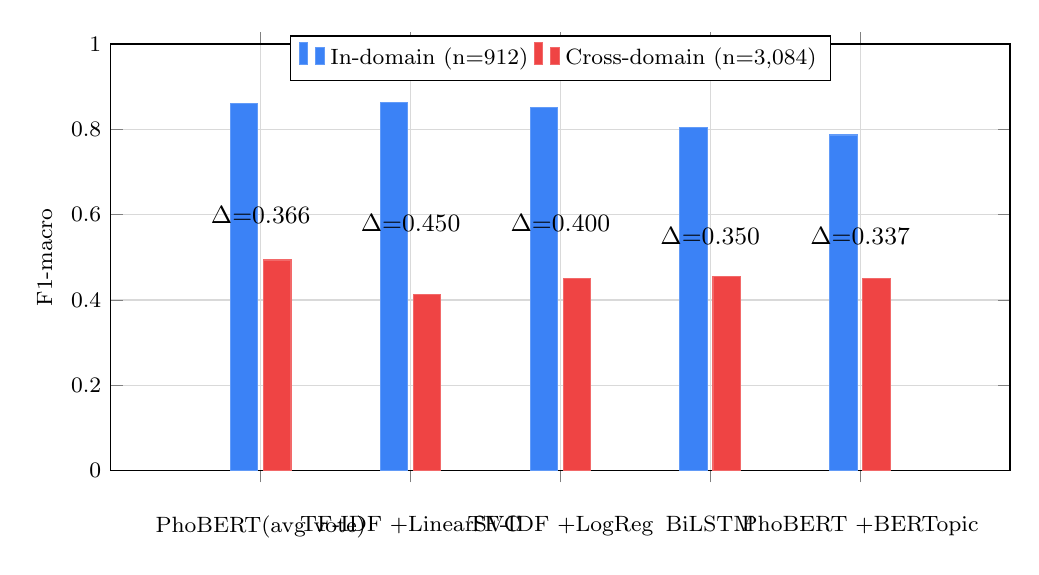
\begin{tikzpicture}
\begin{axis}[
    ybar,
    bar width=0.35cm,
    enlarge x limits=0.25,
    ymin=0, ymax=1,
    ylabel={F1-macro},
    ylabel style={font=\footnotesize},
    xtick=data,
    xticklabels={
        {PhoBERT\\(avg vote)},
        {TF-IDF +\\LinearSVC},
        {TF-IDF +\\LogReg},
        {BiLSTM},
        {PhoBERT +\\BERTopic}
    },
    tick label style={font=\fontsize{8}{9}\selectfont},
    x tick label style={rotate=0, anchor=north, yshift=-0.3cm},
    legend style={
        at={(0.5,1.02)},
        anchor=north,
        legend columns=2,
        font=\footnotesize,
    },
    grid=major,
    grid style={gray!30},
    ytick distance=0.2,
    cycle list={
        {fill=myblue,draw=myblue!80},
        {fill=myred,draw=myred!80},
    },
]

% In-domain (blue)
\addplot coordinates {
    (1, 0.8596)
    (2, 0.8629)
    (3, 0.8504)
    (4, 0.8049)
    (5, 0.7868)
};
\addlegendentry{In-domain (n=912)}

% Cross-domain (red)
\addplot coordinates {
    (1, 0.4937)
    (2, 0.4129)
    (3, 0.4504)
    (4, 0.4549)
    (5, 0.4501)
};
\addlegendentry{Cross-domain (n=3,084)}

% Delta annotations
\node at (axis cs:1,0.60) {\small $\Delta$=0.366};
\node at (axis cs:2,0.58) {\small $\Delta$=0.450};
\node at (axis cs:3,0.58) {\small $\Delta$=0.400};
\node at (axis cs:4,0.55) {\small $\Delta$=0.350};
\node at (axis cs:5,0.55) {\small $\Delta$=0.337};

\end{axis}
\end{tikzpicture}
\end{document}
